\documentclass{article}
\usepackage[utf8]{inputenc}
\usepackage{listings}
\lstset{
  frame=tblr,
  language=C++
}
\usepackage{xcolor}
\usepackage{url}
\usepackage{smartdiagram}
\usesmartdiagramlibrary{additions}
\usepackage{hyperref}
\hypersetup{
    colorlinks=true,
    linkcolor=blue,
    filecolor=magenta,      
    urlcolor=cyan,
}
 
\title{INF01151 - Sistemas Operacionais II N \\ Trabalho Prático 1 - Relatório de Implementação  }
\author{Fábio de Azevedo Gomes - Cartão 00287696 \\ Octavio Arruda - Cartão 00246622 \\ \textcolor{red}{integrante 3 - cartão 3} \\ \textcolor{red}{integrante 4 - cartão 4}}
\date{October 2020}

% "A equipe deverá produzir um relatório fornecendo os seguintes dados:"
\begin{document}

\maketitle

% "Descrição do ambiente de testes: versão do sistema operacional e distribuição, configuração da máquina (processador(es) e memória) e compiladores utilizados (versões)."
\section{Ambiente de teste e desenvolvimento}
O código desenvolvido faz uso das bibliotecas:
% Bibliotecas usadas
\begin{itemize}
    \item \texttt{sys/socket, sys/types.h, netinet/in.h, arpa/inet.h}
    \\ Todas utilizadas para a implementação da comunicação entre os processos cliente e servidor, utilizando as \texttt{sockets} Unix no protocolo \texttt{TCP}.
    \item \texttt{pthread.h}
    \\ Necessária tanto no cliente quanto no servidor, utilizada para implementar as diversas threads que compoem cada uma dessas aplicações.
    \item \texttt{curses.h}
    \\ Utilizada apenas na aplicação cliente, de forma a permitir a implementação de uma interface amigável e gerenciável sem que seja necessário o uso de "gambiarras" do terminal.
\end{itemize}
e está disponível no  \href{http://github.com/FabioAzevedoGomes/SisOp2}{repositório utilizado} pelo grupo. Abaixo seguem as configurações dos sistemas utilizados por cada integrante
% Integrantes e configuração das máquinas
\begin{itemize}
\item Fábio Gomes: Desenvolveu o código em uma máquina nativa Linux Ubuntu 18.04.5 LTS 64 bits (Ambiente GNOME versão 3.28.2), com 7,7 GiB de memória e um processador Intel® Core™ i7-4500U CPU @ 1.80GHz x 4. Nesta máquina a compilação foi realizada através da \texttt{Makefile} entregue junto ao projeto, utilizando o compilador \texttt{g++} versão 7.5.0. 
\item Octavio Arruda: Desenvolveu o código em uma máquina virtual rodando Linux Ubuntu 20.04.1 LTS 64 bits (Ambiente GNOME versão 3.36.3), com 7,7 GiB de memória e um AMD® Ryzen 3 3200g with radeon vega graphics x 4. Nesta máquina a compilação foi realizada através da \texttt{Makefile} entregue junto ao projeto, utilizando o compilador \texttt{g++} versão 9.3.0. 
\item \textcolor{red}{integrante 3} % TODO configuração da vm / host / compilador
\item \textcolor{red}{integrante 4} % TODO configuração da vm / host / compilador
\end{itemize}

% Explicação e respectivas justificativas a respeito de:
\section{Detalhes de implementação}
Nesta seção serão explicados os detalhes da implementação com relação aos itens citados na especificação, bem como uma visão geral da estrutura do programa.

%(C) Descrição das principais estruturas e funções que a equipe implementou;
\subsection{Estrutura do programa}
Procuramos implementar as aplicações de uma maneira modular, para que possamos adicionar as funcionalidades de forma incremental, e então utilizamos alguns princípios de programação orientada a objetos, tirando proveito da escolha da linguagem \texttt{C++} e a sua adição de classes.
% Dados compartilhados entre aplicações/threads
\subsubsection{Dados}
No arquivo \texttt{data\_types.h} possuímos algumas estruturas que são utilizadas para encapsular os dados transmitidos entre as aplicações cliente e servidor, apresentadas abaixo:
\begin{itemize}
    \item \texttt{Packet}
\end{itemize}
\begin{lstlisting}
typedef struct __packet
{
    uint16_t type;          // Packet type
    uint16_t sqn;           // Sequence number
    uint16_t length;        // Message lenght
    uint64_t timestamp;     // Message timestamp
    const char _payload[];  // Message payload

} packet;
\end{lstlisting}
Esta é a principal estrutura na troca de mensagens entre o cliente e o servidor, funcionando como uma espécie de \textit{header} para os dados enviados. Além de manter o tamanho e o tempo de cada pacote, esta \texttt{struct} também guarda o tipo deste pacote, que pode ser:
\begin{enumerate}
    \item \texttt{PAK\_DATA} Um pacote de dados, com as mensagens dos usuários
    \item \texttt{PAK\_COMMAND} Um pacote de comando, para ações \textit{login} e \textit{disconnect}
    \item \texttt{PAK\_KEEP\_ALIVE} Um pacote para manter a conexão ativa, possui um \texttt{message\_record} vazio
    \item \texttt{PAK\_SERVER\_MESSAGE} Um pacote de mensagens do servidor, contendo mensagens de \textit{login} e \textit{disconnect} que serão apresentadas ao cliente
\end{enumerate}
\begin{itemize}
    \item \texttt{Message Record}
\end{itemize}
\begin{lstlisting}
typedef struct __message_record
{
    char username[23];      // User who sent this message
    uint16_t length;        // Message length
    uint16_t type;          // Message's record type.
    uint64_t timestamp;     // Message timestamp
    const char _message[];  // What the user said

} message_record;
\end{lstlisting}
\par Esta struct é utilizada na troca e recuperação de mensagens trocadas dentro dos grupos. Ao receber mensagens do cliente, o servidor envia para todos conectados no mesmo grupo um \texttt{message\_record} com as informações correspondentes, e também salva este \texttt{message\_record} em um arquivo binário \texttt{.hist} de mesmo nome que o grupo, que contém o histórico das conversas.
\par O campo \texttt{type} é utilizado para distinguir entre mensagens que são enviadas por usuários (\texttt{type = USER\_MESSAGE}) - mensagens no \textit{chat} - e mensagens enviadas pelo servidor (\texttt{type  = SERVER\_MESSAGE}) - como por exemplo \texttt{User <username> has disconnected.} - para que a aplicação cliente possa distingui-las e apresentá-las na tela com a formatação correta até mesmo quando recuperadas do arquivo de histórico.
\subsubsection{Cliente}
    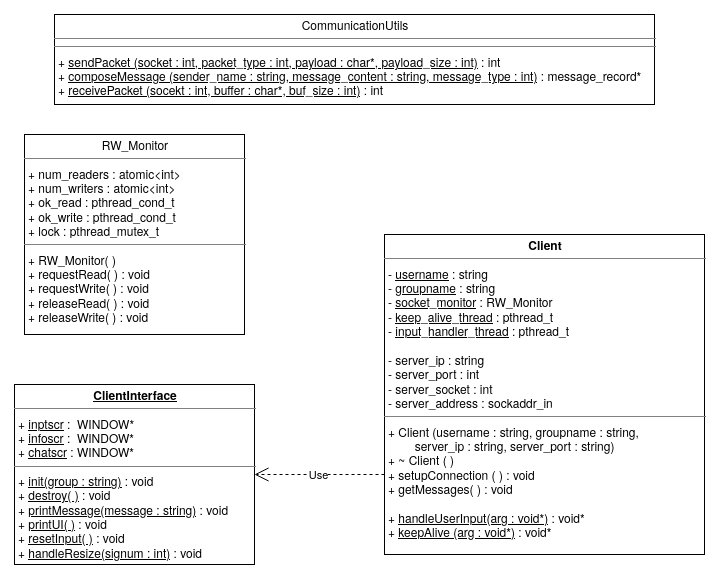
\includegraphics[width=1.0\textwidth]{Client.png}
A aplicação cliente foi desenvolvida de forma a separar a interface que é apresentada ao cliente do núcleo de \textit{threads} que executam para a comunicação com o servidor. Esta classe é relativamente simples, e contém os métodos necessários para o lançamento das \textit{threads} de interação com o servidor.
\par Uma instância de \texttt{Client} é criada pelo método \texttt{main} do arquivo \texttt{clientApp.cpp}, e logo em seguida \texttt{Client::setupConnection} é chamada, passando o controle da aplicação para esta instância.
\par Esta classe faz uso de um monitor, para controle da ordem de escrita na \texttt{socket} como apresentado na seção 2.3, e também requer acesso aos métodos da classe \texttt{CommunicationUtils}, para enviar e receber os pacotes trocados.
\subsubsection{Servidor}
    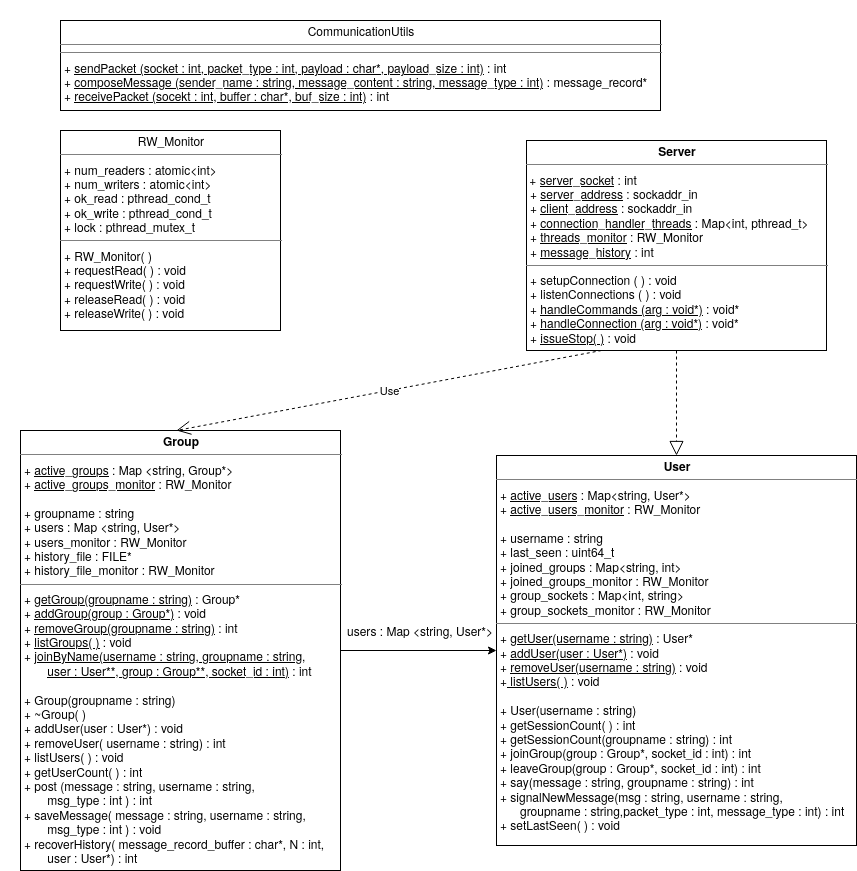
\includegraphics[width=1.0\textwidth]{Server.png}
\par A aplicação servidora apresenta uma estrutura mais complexa, por precisar manipular os objetos do domínio da aplicação - \texttt{Group} e \texttt{User} - enquanto mantendo o controle em uma classe central - \texttt{Server}. A classe \texttt{Server} contém os métodos utilizados para a comunicação com os clientes, em especial os métodos:
\begin{itemize}
    \item \texttt{listenConnections}
    \\ Responsável por escutar na \texttt{socket} principal do servidor, e delegar a uma \textit{thread} executando o método seguite a comunicação.
    \item \texttt{handleConnection}
    \\ Responsável por se comunicar com apenas um cliente, roda em uma \textit{thread} separada de forma que o servidor possa atender múltiplas requisições simultâneamente.
\end{itemize}
os quais executam durante todo o ciclo de vida do mesmo.
\begin{itemize}
    \item \textbf{\texttt{User}}
\end{itemize}
A classe \texttt{User} modela um usuário conectado a um grupo, no qual está ocorrendo a troca de mensagens. Aqui é importante mencionar que um \texttt{User} é diferente de um \texttt{Client}: Segundo a especificação, podemos ter até 2 sessões para um mesmo usuário, em dispositivos diferentes, e portanto podemos ter dois \texttt{Clients} representados no mesmo \texttt{User}. Para estas situações, incluímos a variável \texttt{group\_sockets}, a qual controla quais os clientes que estão mapeados neste usuário, e em qual grupo estão conectados.
\par Incluímos para controle de usuários um \texttt{Map} estático chamado \texttt{active\_users}, o qual contém os nomes e referências de todos os usuários conectados, devidamente protegido por um monitor para permitir o acesso no estilo \textit{Readers and Writers}. Os métodos estáticos da classe \texttt{User} são todos referentes a esse \texttt{Map}.
\par Na instância do cliente, utilizamos os métodos básicos de criação e destruçao, bem como os métodos \texttt{joinGroup} e \texttt{leaveGroup}, os quais realizam a associação e desassociação deste \texttt{User} com um \texttt{Group}, respectivamente.
\par Adicionalmente, temos o método \texttt{say}, o qual envia uma mensagem dita por esse usuário para o \texttt{Group} conectado, e o método \texttt{signalNewMessage}, o qual avisa este usuário de que uma nova mensagem foi enviada em algum de seus grupos conectados, enviando-a para o cliente correto. Como uma observação, estes métodos sempre são chamados em seguida, visto que um usuário faz parte do grupo para o qual está enviando mensagens, e portanto a mensagen será sinalizada a ele e enviada para seu cliente correspondente.  
\begin{itemize}
    \item \textbf{\texttt{Group}}
\end{itemize}
A classe \texttt{Group} modela um grupo que contém usuários, permitindo que a troca de mensagens ocorra de forma consistente entre todos os associados. Similar à classe \texttt{User}, incluímos um \texttt{Map} estático que mantém os nomes e referências para todos os grupos ativos atualemnte, chamado \texttt{active\_groups}, também devidamente protegido por um monitor \textit{Readers-Writers}. 
\par Os métodos estáticos do \texttt{Group} também são aqueles para manipulação dessa estrutura, com exceção do método \texttt{joinByName}, o qual realiza um procedimento mais complexo, requisitando acesso para escrita tanto ao monitor de usuários quanto ao de grupos:
\begin{enumerate}
    \item Procura pelo \textit{username} informado, e se não existir cria um
    \item Procura pelo \textit{groupname} informado, e se não existir cria um
    \item Tenta se juntar ao grupo com o usuário, através de uma chamada do tipo \texttt{user->joinGroup(group, socket)}
    \item Retorna nos ponteiros recebidos referências ao usuário/grupo criado ou obtido.
\end{enumerate}
\par Para o funcionamento da manutenção do histórico, no método construtor de um grupo realizamos uma checagem para verificar se o arquivo de histórico do grupo existe no subdiretório \texttt{hist}, presente no diretório onde o servidor está executando. Neste diretório guardamos arquivos binários no formato \texttt{groupname.hist}, que contém na primeira linha a contagem de mensagens (\texttt{long}), e nas demais estruturas do tipo \texttt{message\_record}, com todas as mensagens enviadas no grupo.
\par Na instância do \texttt{Group}, além dos diversos métodos de controle de usuários, como \texttt{addUser} e \texttt{removeUser}, temos os métodos que realizam a lógica de comunicação: 
\\\texttt{ * post}
\\ Responsável por enviar a mensagem recebida para os usuários ligados a este grupo, através de chamadas a \texttt{User::signalNewMessage}.
\\\texttt{ * saveMessage}
\\ Chamada dentro do método \texttt{post}, salva a mensagem no arquivo de histórico do grupo, em um trecho protegido pelo monitor deste arquivo.
\\\texttt{ * recoverHistory}
\\ Método chamado quando um novo usuário (não cliente) conecta ao grupo, e recupera as últimas \textbf{N} mensagens do arquivo de histórico para serem enviadas a ele.
\\ \textbf{\underline{Observação:}} Os métodos \texttt{User::leaveGroup} e \texttt{Group::removeUser} realizam testes sobre a quantidade de usuários e sessões ativas quando chamados e, a ao verificar que não há mais nenhuma sesssão (no caso de \texttt{User}) ou nenhum usuário (no caso de \texttt{Group}), executam um \texttt{delete(this)}, se removendo da lista de usuários/grupos de forma autônoma.
%(A) Como foi implementada a concorrência no servidor para atender múltiplos clientes;
\subsection{Implementação da concorrência}
A concorrência do servidor foi implementada com auxílio da biblioteca \texttt{pthread.h}, sendo criadas \textit{threads} tanto para comunicação com os usuários quanto para controle do administrador do servidor. Após devido \textit{setup}, a aplicação servidor invoca o método \texttt{Server::listenConnections}, o qual dá início à concorrência.
\par Este método é responsável por, primeiramente, iniciar uma \textit{thread} para executar a rotina \texttt{Server::handleCommands}, cujo único propósito é capturar comandos do administrador do servidor, permitindo que ele execute ações como listar os usuários e grupos. Estes comandos foram utilizados para facilitar o processo de \textit{debugging} da aplicação.
\par Após iniciada esta \textit{thread}, o método entra em um \textit{loop} \texttt{while} no qual espera por conexões ou pelo encerramento do servidor pelo administrador. Este \texttt{while} está apresentado abaixo, junto com uma explicação de seu funcionamento;
\\
\begin{lstlisting}[xleftmargin=-.05\textwidth, xrightmargin=-.05\textwidth]
while(!stop_issued && (client_socket = 
                       accept(server_socket, 
                             (struct sockaddr*)&client_address, 
                             (socklen_t*)&sockaddr_size)) )
{
      // Start new thread for new connection
        pthread_t comm_thread;
        
        // Get reference to client socket
        new_socket = (int*)malloc(sizeof(int));
        *new_socket = client_socket;
        
        // Set the keep-alive timer on the socket
        if (setsockopt(client_socket, 
                       SOL_SOCKET, 
                       SO_RCVTIMEO, 
                       (const char*)&timeout_timer, 
                       sizeof(timeout_timer)) < 0 )
         throw std::runtime_error(appendErrorMessage(
                    "Error setting socket options"));
        
        // Spawn new thread for handling that client
        if (pthread_create( &comm_thread, 
                         NULL, 
                         handleConnection, 
                         (void*)new_socket) < 0)
        {
         // Close socket if no thread was created
         close(client_socket);
        }
        
        // Request write rights
        threads_monitor.requestWrite();
        
        // Add thread to list of connection handlers
        connection_handler_threads.insert(
            std::make_pair(*new_socket, comm_thread));
        
        // Release write rights
        threads_monitor.releaseWrite();
}
\end{lstlisting}
\par Este trecho de código espera por conexões dos clientes e ao receber uma, realiza uma tentativa de criação de uma nova \textit{thread}, que será responsável pela comunicação com o novo cliente (Através do método \texttt{Server::handleConnection}). Esta nova \textit{thread} recebe como parâmetro o novo descritor de \texttt{socket} do cliente para que possa realizar a troca de mensagens. Neste mesmo trecho de código a \texttt{socket} é configurada para que possua um \textit{timeout}, conforme o tempo definido no arquivo \texttt{constants.h}.
\par Se a \textit{thread} for criada com sucesso, ela é adicionada à lista de \textit{threads} responsáveis por comunicação com clientes de forma a manter o controle de todas as \textit{threads}. Quando o administrador do servidor envia um comando de \texttt{stop}, este \textit{loop} é terminado e o trecho de código seguinte é executado;
\\
\begin{lstlisting}
// Wait for all threads to finish
for (std::map<int, pthread_t>::iterator i = 
            connection_handler_threads.begin();
            i != connection_handler_threads.end(); ++i)
{

    // Get the thread reference
    pthread_join(i->second, NULL);

    // Save the thread number
    thread_socket = i->first;
    
    // Remove this ended thread from the thread list
    connection_handler_threads.erase(thread_socket);
}
\end{lstlisting}
\par Neste trecho, por fim, a \textit{thread} principal de execução espera todas as demais que ainda estão em execução através da primitiva \texttt{pthread\_join}, de forma que todas possam encerrar corretamente e o servidor retorne sem erros ou \textit{threads} perdidas.

%(B) Em quais áreas do código foi necessário garantir sincronização no acesso a dados;
\subsection{Implementação da sincronização}
A sincronização de \textit{threads} foi necessária tanto na implementação do cliente quanto na implementação do servidor, e apareceu de duas maneiras principais:
\begin{itemize}
    \item \textbf{Acesso a dados concorrente:} Foi preciso implementar estruturas de controle vistas na primeira área da disciplina para controlar a leitura e escrita em \textit{buffers} e arquivos compartilhados entre \textit{threads}.
    
    \item \textbf{Sincronização de \textit{threads}:} Como tanto a aplicação cliente quanto a aplicação servidor utiliza múltiplas \textit{threads} foi necessário manter controle de quais \textit{threads} estão vivas a cada momento, e no encerramento dessas duas aplicações precisamos encerrar, de forma segura, todas as \textit{threads} ativas.
\end{itemize}
\par Para o caso de acesso aos dados compartilhados, implementamos uma classe chamada \texttt{RW\_Monitor} utilizando algumas definições da biblioteca \texttt{pthread.h}, cujo protótipo está apresentado abaixo, e que implementa, utilizando as variáveis de condição \texttt{ok\_read}, \texttt{ok\_write} e um \texttt{mutex} a proteção para o problema dos leitores e escritores, como apresentado em aula. Esta classe foi instanciada para cada dado comparilhado que precisava ser protegido, e garantindo a proteção desses dados durante a execução do servidor através de \texttt{requests} e \texttt{releases} desses monitores.
\\
\begin{lstlisting}
class RW_Monitor
{
    public:
    std::atomic<int> num_readers, num_writers;
    pthread_cond_t ok_read, ok_write;
    pthread_mutex_t lock;

    RW_Monitor();

    void requestRead();

    void requestWrite();

    void releaseRead();

    void releaseWrite();
};
\end{lstlisting}
\par O encerramento das aplicações cliente e servidor é feito através de uma variável compartilhada entre todas as \textit{threads}, em ambas as aplicações chamada \texttt{stop\_issued}, que sinaliza o encerramento realizado por parte do usuário. Esta variável é do tipo \texttt{std::atomic<bool>} garantindo o acesso atômico à mesma, garantindo uma camada extra de proteção concorrente.

% Implementação da sincronização na aplicação cliente
\subsubsection{Sincronização no cliente}
\par No cliente, o trecho de código abaixo é responsável por sincronizar todas as \textit{threads} no encerramento. 
\par Após realizar a sinalização de parada, a \textit{thread} principal espera pela \textit{thread} de \textit{input} do usuário para seguir em frente, que encerrará após o próximo \textit{Enter} do usuário.
\par Feito isso, utilizamos uma chamada \texttt{pthread\_cancel} para acordar a \textit{thread} de mensagens de \textit{keep-alive}, para que possa encerrar de forma correta e nos juntamos a ela através de outro \texttt{pthread\_join}.
\\
\begin{lstlisting}
// Signal threads to stop
stop_issued = true;

// Wait for input handler thread to finish
pthread_join(Client::input_handler_thread,NULL);

// Wake up the keep-alive thread from it's sleep
pthread_cancel(Client::keep_alive_thread);
pthread_join(Client::keep_alive_thread, NULL);
\end{lstlisting}
\par Além disso, o cliente também possui um monitor para a escrita na \texttt{socket}, de forma que a \textit{thread} que captura o \textit{input} do usuário e a \textit{thread} que envia mensagens de \textit{keep-alive} não realizem este acesso concorrentemente
% Implementação da sincronização na aplicação servidora
\subsubsection{Sincronização no servidor}
\par O servidor, devido às suas características de \textit{multi-threading} foi onde a necessidade de sincronização esteve mais presente, de forma a garantir que os diversos clientes conectados não realizassem operações conflitantes nas estruturas de controle salvas.
\begin{itemize}
    \item \textbf{Server class}
        \\Na classe principal do servidor, utilizamos apenas um monitor, de nome \texttt{threads\_monitor}. Este monitor protege a variável \texttt{connection\_handler\_threads}, a qual é um mapa entre um valor \texttt{int}(o descritor da socket na qual aquela \textit{thread} escuta) e um \textit{handle} \texttt{pthread\_t}(Descritor daquela \textit{thread}).
    \item \textbf{User class}
        \\Na classe que modela os usuários conectados ao \textit{chat} utilizamos 3 monitores diferentes:
        \begin{itemize}
            \item \texttt{active\_users\_monitor} 
            \item \texttt{joined\_groups\_monitor}
            \item \texttt{group\_sockets\_monitor}
        \end{itemize}
        \par O primeiro monitor, \texttt{active\_users\_monitor}, é de caráter estático, e protege o mapa estático de referências de usuários, \texttt{active\_users}, através do qual o controle de usuários conectados ao chat é realizado.
        \par O segundo monitor, \texttt{joined\_groups\_monitor}, é relacionado à instância de usuário, e protege o mapa de grupos nos quais este cliente está conectado, denominado \texttt{joined\_groups}.
        \par O terceiro monitor, \texttt{group\_sockets\_monitor}, mantém protegido o mapa \texttt{group\_sockets}, o qual mantém uma forma de endereçar os clientes através dos quais este usuário está conectado, a qual grupo cada um deles está associado.
    \item \textbf{Group class}
    \\Na classe que modela os grupos utilizamos novamente 3 monitores, um deles também estático:
    \begin{itemize}
        \item \texttt{active\_groups\_monitor}
        \item \texttt{users\_monitor}
        \item \texttt{history\_file\_monitor}
    \end{itemize}
    \par O primeiro e o segundo monitor - \texttt{active\_groups\_monitor} e \texttt{users\_monitor}, respectivamente - são similares àqueles na classe do usuário, e mantém protegidos os mapas que controlam os grupos que estão ativos e os usuários conectados em cada um deles - \texttt{active\_groups} e \texttt{users}.
    \par O terceiro monitor, \texttt{history\_file\_monitor}, protege o acesso ao arquivo de histórico do grupo, onde as mensagens passadas são salvas. Este monitor garante que não serão feitas duas escritas no arquivo de histórico ao mesmo tempo, prevenindo a corrupção dos dados.
\end{itemize}

%(D) Explicar o uso das diferentes primitivas de comunicação;
\subsection{Implementação da comunicação}
\par A comunicação entre cliente e servidor foi realizada através do uso de primitivas do \textit{header} \texttt{sys/socket.h}, encapsuladas em uma classe \texttt{CommunicationUtils}, encarregada de criar e popular os pacotes que são trocados entre as aplicações, enviando-os através da primitiva \texttt{send}:
\\
\begin{lstlisting}[xleftmargin=-.1\textwidth, xrightmargin=-.1\textwidth]
// Send packet
if ( (bytes_sent = send(socket, data, packet_size, 0)) <= 0)
 throw std::runtime_error(
       appendErrorMessage("Unable to send message to server"));
\end{lstlisting}
e recebendo-os através da primitiva \texttt{recv}:
\begin{lstlisting}
// While header doesn't arrive and socket is open
while (read_bytes >= 0 && total_bytes < header_size && 
      (read_bytes = 
      recv(socket, 
           buffer + total_bytes, 
           header_size - total_bytes, 0)) > 0)
{
    // If data has arrived, increase total
    if (read_bytes > 0) total_bytes += read_bytes;
    // If socket was closed, reset total
    else total_bytes = -1;
}
\end{lstlisting}
\subsubsection{Cliente}
\par Na implementação do cliente, seguimos o \textit{flowchart} apresentado em aula para a comunicação com \texttt{sockets} \texttt{TCP}, como pode ser visto abaixo:
\begin{center}
    \smartdiagramset{
        uniform color list = white!60!black for 5 items,
        back arrow disabled = true,
        additions = {
            additional arrow color = gray,
            additional arrow tip=stealth,
            additional arrow line width=2.8pt,
        }
    }
    \smartdiagramadd[flow diagram:horizontal]{socket, connect, write, read, close}{}
    \smartdiagramconnect{->}{module4/module3}
\end{center}%
\par Os 2 primeiros itens foram encapsulados no método \texttt{Client::setupConnection()}, apresentado abaixo, o qual realiza esta criação da \texttt{socket}, no modo \texttt{TCP} (\texttt{SOCK\_STREAM}) e preenche a estrutura do servidor, utilizando a porta informada na linha de comando. Feito isto, o cliente realiza uma tentativa de conexão ao servidor utilizando a primitiva \texttt{connect}, utilizando esta \texttt{socket} criada e a estrutura preenchida
\\
\begin{lstlisting}[xleftmargin=-.1\textwidth, xrightmargin=-.1\textwidth]
    int payload_size;
    
    // Create socket
    if ( (server_socket = socket(AF_INET, SOCK_STREAM, 0)) < 0)
     throw std::runtime_error(
                appendErrorMessage("Error during socket creation"));
    
    // Fill server socket address
    server_address.sin_family = AF_INET;
    server_address.sin_port   = htons(server_port);
    server_address.sin_addr.s_addr = inet_addr(server_ip.c_str());
    
    // Try to connect to remote server
    if (connect(server_socket, 
               (struct sockaddr *)&server_address, 
               sizeof(server_address)) < 0)
     throw std::runtime_error(
                appendErrorMessage("Error connecting to server"));
\end{lstlisting}
\par Realizado este processo de \textit{setup} e conexão com sucesso, o cliente imediatamente envia para o servidor a primeira mensagem - \textit{login}, a qual contém as informações sobre o usuário e grupo deste cliente.
\\
\begin{lstlisting}[xleftmargin=-.1\textwidth, xrightmargin=-.1\textwidth]
    // Prepare message record with login information
    login_record = CommunicationUtils::composeMessage(
      username, std::string(groupname), LOGIN_MESSAGE);

    // Sends the command packet to the server
    CommunicationUtils::sendPacket(server_socket,
                                   PAK_COMMAND, 
                                   (char*)login_record,
                                   sizeof(*login_record) +
                                   login_record->length); 

    // Free login record
    free(login_record);


\end{lstlisting}

\par A partir deste ponto, a aplicação cliente é separada em duas \textit{threads}, responsáveis por receber \textit{input} do usuário e obter mensagens do servidor.
\begin{itemize}
\item \textbf{Obtenção de mensagens vindas do servidor}
\\
\par A \textit{thread} responsável pelas mensagens do servidor fica em um \textit{loop} na função \textit{void Client::getMessages()}, cuja condição de laço é apresentada abaixo:
\\
\begin{lstlisting}[xleftmargin=-.1\textwidth, xrightmargin=-.1\textwidth]
    // Wait for messages from the server
while(!stop_issued && 
     (read_bytes = 
          CommunicationUtils::receivePacket(server_socket, 
                                            server_message,
                                            PACKET_MAX)) > 0)
\end{lstlisting}
\par A aplicação cliente espera por mensagens vindas do servidor, tentando ler apenas o \textit{header} do pacote, e ao obter este dado compõe o \textit{payload} da mensagem recebida em uma espécie de \textit{busy-waiting}, seguindo então para o processo de decodificação.

\item \textbf{Obtenção de \textit{input} do usuário}
\\ A \textit{thread} responsável por obter mensagens do usuário permanece em um \textit{loop} capturando o que é digitado, dentro da função \texttt{void *Client::handleUserInput(void* arg)}. Obtida a mensagem, é feita uma chamada ao método \\
\texttt{CommunicationUtils::sendPacket(server\_socket, PAK\_DATA, payload, payload\_size)}, que a envia ao servidor.
\end{itemize}
\subsubsection{Servidor}
No servidor utilizamos, novamente, o \textit{flowchart} de comunicação \texttt{TCP} apresentado em aula. 
\\
\begin{itemize}
    \item \textit{\textbf{Setup}}\\
O \textit{setup} segue o diagrama abaixo:
\\
\begin{center}
    \smartdiagramset{
        uniform color list = white!60!black for 4 items,
        back arrow disabled = true,
        additions = {
            additional arrow color = gray,
            additional arrow tip=stealth,
            additional arrow line width=2.8pt,
        }
    }
    \smartdiagramadd[flow diagram:horizontal]{socket, bind, listen, accept}{}
\end{center}%
e é implementado pela função \texttt{void Server::setupConnection()}, como apresentado, com um passo extra de configuração da \texttt{socket} para que reutilize o mesmo endereço de porta:
\\
\begin{lstlisting}[xleftmargin=-.1\textwidth, xrightmargin=-.1\textwidth]
// Create socket
if ( (server_socket = socket(AF_INET, SOCK_STREAM, 0)) < 0)
 throw std::runtime_error(
            appendErrorMessage("Error during socket creation"));

// Prepare server socket address
server_address.sin_family = AF_INET;
server_address.sin_addr.s_addr = INADDR_ANY;
server_address.sin_port = htons(SERVER_PORT);

// Set socket options
int yes = 1;
if (setsockopt(server_socket, 
               SOL_SOCKET, 
               SO_REUSEADDR, 
               &yes, 
               sizeof(yes)) == -1)
 throw std::runtime_error(
            appendErrorMessage("Error setting socket options"));

// Bind socket
if ( bind(server_socket, 
         (struct sockaddr *)&server_address, 
          sizeof(server_address)) < 0)
    throw std::runtime_error(
               appendErrorMessage("Error during socket bind"));
\end{lstlisting}
Feito este \textit{setup}, o servidor inicia uma \textit{thread} para obter comandos do administrador, e troca para a função \texttt{void Server::listenConnections()}, onde o \textit{loop} de aceitação de conexões ocorre como apresentado na seção 2.2.
\item \textbf{Comunicação}
\par Ao receber uma nova conexão, o servidor cria uma \textit{thread} para lidar com aquela conexão, salvando-a no mapa e retornando ao \textit{loop}. A comunicação segue a segunda parte do \textit{flowchart}, com cada \textit{thread} de cada cliente realizando estas operações:
\begin{center}
    \smartdiagramset{
        uniform color list = white!60!black for 4 items,
        back arrow disabled = true,
        additions = {
            additional arrow color = gray,
            additional arrow tip=stealth,
            additional arrow line width=2.8pt,
        }
    }
    \smartdiagramadd[flow diagram:horizontal]{read, write, close}{}
    \smartdiagramconnect{->}{module2/module1}
\end{center}%
A \textit{thread} criada para a comunicação com o cliente é denominada \texttt{Server::handleConnection}, e compõe o coração da aplicação servidora - é nela em que todas as comunicações com um cliente ocorrem - recebendo e enviando \texttt{packets} atraés da sua \texttt{socket}. Abaixo temos uma versão simplificada desta função, de forma a apresentar seus pontos principais:
\\
\begin{lstlisting}[xleftmargin=-.2\textwidth, xrightmargin=-.2\textwidth]
while((read_bytes = recv(socket, client_message, PACKET_MAX, 0)) > 0)
{
    // Decode received data into a packet structure
    packet* received_packet = (packet *)client_message;

    // Decide action according to packet type
    switch (received_packet->type)
            ...

    // Clear the buffers
    bzero((void*)client_message, PACKET_MAX);
    bzero((void*)message_records, PACKET_MAX * Server::message_history);
}
\end{lstlisting}
\par O \textit{loop} de execução desta \textit{thread} é o esperado: recebe mensagens dos clientes até que o servidor encerre, o cliente associado encerre ou o \textit{timeout} seja atingido. Vale notar aqui que a variável \texttt{socket} é aquela recebida como parâmetro quando a função \texttt{Server::listenConnections} cria a \textit{thread}, e de-referenciada no início da execução da \textit{thread} como apresentado:
\begin{lstlisting}
    int socket = *(int*)arg; // Client socket
\end{lstlisting}
\par Dentro deste \textit{loop} é executado um \texttt{switch-case}, o qual decide a ação tomada pela \textit{thread} de comunicação baseado no tipo de pacote que foi recebido do usuário. Existem 3 tipos de pacotes que são recebidos:
\begin{enumerate}
    \item PAK\_DATA
    \item PAK\_COMMAND
    \item PAK\_KEEP\_ALIVE
\end{enumerate}
%
\begin{itemize}
    \item \textbf{PAK\_DATA}
\end{itemize}
\par Pacotes de dados que são recebidos pela \textit{thread} de comunicação contém mensagens que estão sendo enviadas pelo usuário para serem "postadas" no \textit{chat} do grupo conectado. A \textit{thread} então utiliza o método \texttt{say} da instância do usuário conectado, delegando aos objetos do domínio a lógica de \textit{broadcast} desta mensagem, da forma apresentada na seção 2.1.3
\par Abaixo vemos este procedimento que é executado dentro do \texttt{case}:
\begin{lstlisting}[xleftmargin=-.1\textwidth, xrightmargin=-.1\textwidth]
case PAK_DATA:   // Data packet

    // Decode received message into a message record
    read_message = (message_record*)received_packet->_payload;

    // If user and group still exist
    if (user != NULL && group != NULL && !stop_issued)
    {
        // Update user's last seen variable
        user->setLastSeen();

        // Say message to the group
        user->say(read_message->_message, group->groupname);
    }
    
    break;
\end{lstlisting}
\begin{itemize}
    \item \textbf{PAK\_COMMAND}
\end{itemize}
\par Pacotes de comando são recebidos do cliente quando o mesmo está tentando realizar uma operação de \textit{login}, e contém o nome de usuário do cliente no campo \texttt{username} e o nome do grupo que deseja ingressar no corpo do \texttt{message\_record}: \texttt{\_message}.
\par O processo de \textit{login}, então, é realizado pela função \texttt{Group::joinByName}, a qual encapsula os passos de :
\begin{enumerate}
    \item Obtenção de referência ao usuário
    \item Obtenção de referência ao grupo
    \item Associação das instâncias de usuário e gurpo
\end{enumerate}
de forma protegida por monitores, garantindo a proteção de seções críticas do código.

\begin{itemize}
    \item \textbf{PAK\_KEEP\_ALIVE}
\end{itemize}
\par Por fim, o último tipo de pacote que o servidor pode receber é o pacote para implementação do sistema de \textit{keep-alive} o qual, ao ser recebido, "reseta" o tempo de \textit{timeout} da \texttt{socket}. Este pacote não tem nenhuma informação associada a ele, e é composto por um \texttt{message\_record} de corpo vazio.
\\
%
\par No final da conexão (ao encerrar o \textit{loop} de recepção e troca de mensagens) a \textit{thread} realiza uma serie de testes para verificar o motivo da conexão ter encerrado, e também realiza a desassociação do usuário com o grupo, enviando uma mensagem de \textit{Disconnect} para o grupo caso esta seja a última sessão do usuário naquele grupo. Estes procedimentos estão apresentados abaixo:
\begin{lstlisting}[xleftmargin=-.2\textwidth, xrightmargin=-.2\textwidth]
// Leave group with this user
if (user != NULL) user->leaveGroup(group, socket);

// Check if connection ended due to timeout
if(errno == EAGAIN || errno == EWOULDBLOCK)
{
    // If so, close the connection for good
    close(socket);
}

// Request read rights
User::active_users_monitor.requestRead();
Group::active_groups_monitor.requestRead();

// Check if the user doesn't exist, 
// the group still exists, 
// and server was not stopped
if (User::active_users.find(username) == User::active_users.end()   &&
    Group::active_groups.find(groupname) != Group::active_groups.end() &&
    !stop_issued)
{
    message = "User [" + username + "] has disconnected.";
    group->post(message ,username, SERVER_MESSAGE);
}

// Release read rights
User::active_users_monitor.releaseRead();
Group::active_groups_monitor.releaseRead();
\end{lstlisting}
e por fim se remove da lista de \textit{threads} compartilhada do servidor, dado que não foi sinalizada a parada (Nesse caso, o próprio método \texttt{Server::listenConnections} se encarrega de remover as \textit{threads} da lista), dando fim à conexão previamente estabelecida
\\
\begin{lstlisting}
if (!stop_issued)
{
    // Request write rights
    threads_monitor.requestWrite();

    // Remove itself from the threads list
    connection_handler_threads.erase(socket);

    // Release write rights
    threads_monitor.releaseWrite();
}
\end{lstlisting}
\end{itemize}
% Inclusão no relatório de uma descrição dos problemas que a equipe encontrou durante a implementação e como estes foram resolvidos (ou não).
\section{Problemas encontrados durante a implementação}
Encontramos dois problemas principais durante a implementação da aplicação, concentrados principalmente na aplicação servidor:
\subsection{\textit{Deadlocks} e ordem de execução das operações}
\par Dado que o servidor é implementado majoritariamente utilizando a arquitetura \textit{multi-threaded}, tivemos muitas dificuldades que surgiram pela falta de determinismo na execução, bem como a grande quantidade de possíveis ordens que as \textit{threads} podiam tomar em cada situação.
\par Por consequência, tivemos que lidar com uma grande quantidade de \textit{Mandelbugs}, o que foi resolvido através da simulação mental das possíveis execuções da aplicação (como "testes de mesa") e desenhos e anotações sobre as linhas de execução e os dados que estavam acessando e criando/destruindo. Um exemplo disto pode ser visto no trecho de código abaixo, que gerava um \texttt{SIGSEGV} somente quando uma ordem específica de operações era realizada:
\\
\begin{lstlisting}[numbers=left, stepnumber=1]
// Get reference to group
group = Group::getGroup(login_payload_buffer->groupname)

// Get reference to user
user = User::getUser(login_payload_buffer->username))

    ...

// Try to join that group with this user
if (user->joinGroup(group, socket) != 0)
{
    ...
\end{lstlisting}
\par Neste trecho, fomos capazes de detectar a causa ao realizar uma inspeção utilizando simulação da execução no papel:
\begin{enumerate}
    \item Suponha que, atualmente, o servidor possua apenas 1 grupo ativo com apenas 1 usuário conectado.
    \item Agora, suponha que um segundo usuário conecta, e tenta se conectar ao mesmo grupo, porém é preemptado logo após a execução da linha 2.
    \item Suponha, então, que a \textit{thread} responsável pelo usuário que estava conectado volte a executar, e este usuário desconecte-se do grupo, deixando o grupo com 0 usuários e por consequência removendo sua instância da lista de grupos.
    \item Agora quando a execução retornar ao usuário que estava conectando, ele possui uma referência inválida para o grupo, e ao tentar executar o código na linha 10 irá gerar um \texttt{SIGSEGV}.
\end{enumerate}
A forma como isto foi resolvido foi encapsular todo o processo de obtenção de referência para usuários e grupos e associação em um único método, protegido pelos monitores correspondentes das listas de usuários e de grupos, como em :
\begin{lstlisting}
Group::joinByName(username, groupname, 
                  &user, &group,  socket)
\end{lstlisting}
\par Também tivemos que lidar com situações onde, ao terminar o servidor, a aplicação não encerrava graciosamente, e "pendurava" a espera de outras \textit{threads}. Após inspeção do código, notamos que isto ocorria devido a um \textit{deadlock} no momento do encerramento, onde a \textit{thread} principal de execução havia requisitado acesso à lista de \textit{threads} para realizar um \texttt{pthread\_join} (Utilizando um monitor) e a \textit{thread} sendo encerrada estava, também, requisitando acesso a esta lista para remover sua entrada  (de forma a não acumular \textit{threads} inuteis na lista), causando um \textit{deadlock}.
\subsection{Gerenciamento de memória em dados compartilhados}
\par Novamente devido a estarmos trabalhando com múltiplas \textit{threads}, encontramos diversos problemas relacionados à gerência de instâncias de objetos compartilhadas entre elas, apresentados na forma de falta de gerência - Memória não era liberada, ou pelo menos não completamente, e eventualmente gerava um acúmulo que causava um \texttt{SIGSEGV} na aplicação - e também na gerência pela \textit{thread} incorreta - \textit{Thread} liberava a memória antes do momento correto, o que causava outra \textit{thread} que ainda precisava deste recurso a acessar uma posição inválida.
\par Resolvemos estes problemas utilizando aplicações externas para \textit{debug} da aplicação, como \texttt{valgrind} e \texttt{gdb} para identificar onde estes recursos estavam sendo liberados e por qual \textit{thread}, o que nos permitiu "caçar" todos os lugares onde estes erros aconteciam e corrigi-los, através de testes de validação (\textit{obj != NULL}) e manutenção de referencias (Criar estruturas para guardar todas as referências, de forma que elas não se percam em uma \textit{thread} encerrante).

\end{document}
